% THIS IS SIGPROC-SP.TEX - VERSION 3.1
% WORKS WITH V3.2SP OF ACM_PROC_ARTICLE-SP.CLS
% APRIL 2009
%
% It is an example file showing how to use the 'acm_proc_article-sp.cls' V3.2SP
% LaTeX2e document class file for Conference Proceedings submissions.
% ----------------------------------------------------------------------------------------------------------------
% This .tex file (and associated .cls V3.2SP) *DOES NOT* produce:
%       1) The Permission Statement
%       2) The Conference (location) Info information
%       3) The Copyright Line with ACM data
%       4) Page numbering
% ---------------------------------------------------------------------------------------------------------------
% It is an example which *does* use the .bib file (from which the .bbl file
% is produced).
% REMEMBER HOWEVER: After having produced the .bbl file,
% and prior to final submission,
% you need to 'insert'  your .bbl file into your source .tex file so as to provide
% ONE 'self-contained' source file.
%
% Questions regarding SIGS should be sent to
% Adrienne Griscti ---> griscti@acm.org
%
% Questions/suggestions regarding the guidelines, .tex and .cls files, etc. to
% Gerald Murray ---> murray@hq.acm.org
%
% For tracking purposes - this is V3.1SP - APRIL 2009

\documentclass{acm_proc_article-sp}
\usepackage{multicol}
\begin{document}

\title{NIJI : Towards Provable and Scalable Anonymity in Mobile Cloud}



%
% You need the command \numberofauthors to handle the 'placement
% and alignment' of the authors beneath the title.
%
% For aesthetic reasons, we recommend 'three authors at a time'
% i.e. three 'name/affiliation blocks' be placed beneath the title.
%
% NOTE: You are NOT restricted in how many 'rows' of
% "name/affiliations" may appear. We just ask that you restrict
% the number of 'columns' to three.
%
% Because of the available 'opening page real-estate'
% we ask you to refrain from putting more than six authors
% (two rows with three columns) beneath the article title.
% More than six makes the first-page appear very cluttered indeed.
%
% Use the \alignauthor commands to handle the names
% and affiliations for an 'aesthetic maximum' of six authors.
% Add names, affiliations, addresses for
% the seventh etc. author(s) as the argument for the
% \additionalauthors command.
% These 'additional authors' will be output/set for you
% without further effort on your part as the last section in
% the body of your article BEFORE References or any Appendices.

\numberofauthors{6} %  in this sample file, there are a *total*
% of EIGHT authors. SIX appear on the 'first-page' (for formatting
% reasons) and the remaining two appear in the \additionalauthors section.
%
\author {
% You can go ahead and credit any number of authors here,
% e.g. one 'row of three' or two rows (consisting of one row of three
% and a second row of one, two or three).
%
% The command \alignauthor (no curly braces needed) should
% precede each author name, affiliation/snail-mail address and
% e-mail address. Additionally, tag each line of
% affiliation/address with \affaddr, and tag the
% e-mail address with \email.
%
% 1st. author
\alignauthor
Aravindan Balan\\
       \email{aravindan@cs.ucla.edu}
% 2nd. author
\alignauthor
Johnathan Chai\\
       \email{johnathanchai@ucla.edu}      
% 3rd. author
\alignauthor
Swati Katta\\
       \email{swati1591@cs.ucla.edu}
       \and    
% 4th. author
\alignauthor
Vijay Kristipati\\
       \email{kvijay78@gmail.com}            
% 5th. author
\alignauthor 
Joshua Joy\\
       \email{jjoy@cs.ucla.edu}
% 6th. author
\alignauthor 
Mario Gerla\\
       \email{gerla@cs.ucla.edu}
       \and
\alignauthor 
University of California Los Angeles\\
}
% There's nothing stopping you putting the seventh, eighth, etc.
% author on the opening page (as the 'third row') but we ask,
% for aesthetic reasons that you place these 'additional authors'
% in the \additional authors block, viz.

% Just remember to make sure that the TOTAL number of authors
% is the number that will appear on the first page PLUS the
% number that will appear in the \additionalauthors section.

\maketitle
\begin{abstract}
\vspace{1 mm}
In the modern age of the internet, users are becoming concerned about the privacy of their information and actions. To help accomplish this, the Dining Crypotographers network (DC-net) scheme allows users to communicate anonymously in a network. Often we also require receiver anonymity and a sense of confidentiality. In order to achieve this, we make use of a novel technique using encryption. Our work combines the benefits of DCNets and various encryption schemes for a practical anonymous messaging network on mobile devices. The functionality of our proposed network is verified using ns-3 simulations. With optimization, this protocol can be implemented in a mobile application.

\end{abstract}


\keywords{Peer-to-Peer, Anonymity, DC-net, Privacy, Mobile Cloud  } % NOT required for Proceedings

\section{Introduction}
\vspace{1 mm}
Online privacy has become an important topic as internet use continues to grow rapidly over the past decade. With the ability to wiretap communications, the government or other entities can maintain surveillance on civilians, both domestically and internationally. This imposes a threat towards the freedom of speech because government leaders can identify and arrest dissenters. Though software on an Internet Service Provider (ISP) may have a difficult time revealing contents of encrypted messages, it can still trace down the sender. There are other applications such as protecting personal medical information that could be compromised by the lack of anonymity and privacy over internet channels. This paper will introduce previous work in the area of anonymous messaging networks, and then propose a protocol that draws upon the strengths of different existing designs. Using the ns-3 network simulator, we are able to validate and measure the performance of the new protocol.
 
In the hypothetical Dining Crypotographers network (DC-net), three crypotographers at dinner want to learn if someone at their table paid for the bill, or if it was arranged by a third party such as the U.S. National Security Agency (NSA) \cite{chaum}. Each cryptographer flips a coin and shares the result only with the diner sitting to his right at the table. Then each diner publicly states the logical XOR of the two coin flips he sees. However, the cryptographer who paid for the dinner will state the opposite result. Thus, if an odd number of differences is stated, then one of the cryptographers paid for the dinner; otherwise, if the number is even, then the NSA has paid instead. The advantage of this procedure is that the cryptographer who paid for the dinner can remain anonymous.
 
\section{Methodology}
\vspace{1 mm}

\subsection{Basic Principle: DCNets}

Suppose there are 3 nodes in the network A, B, C. All of them will have a public-private key pair and an ID. During initialization of the secret symmetric key, nodes exchange public keys. Next, messages are sent between all node pairs using public key encryption. The messages will be decrypted using the receiver's private key. The message contains the ID and Diffie Hellman values p, q, g, which are encrypted using receivers public key. The symmetric keys are used for all further communication between nodes. The sender can broadcasts a message to all nodes and the receivers will try to decrypt it using their symmetric keys. However, only the intended receiver will be able to decrypt the message. To maintain anonymity, all the encrypted messages need to be sent using the DC-net concept.

\begin{figure*}
\centering
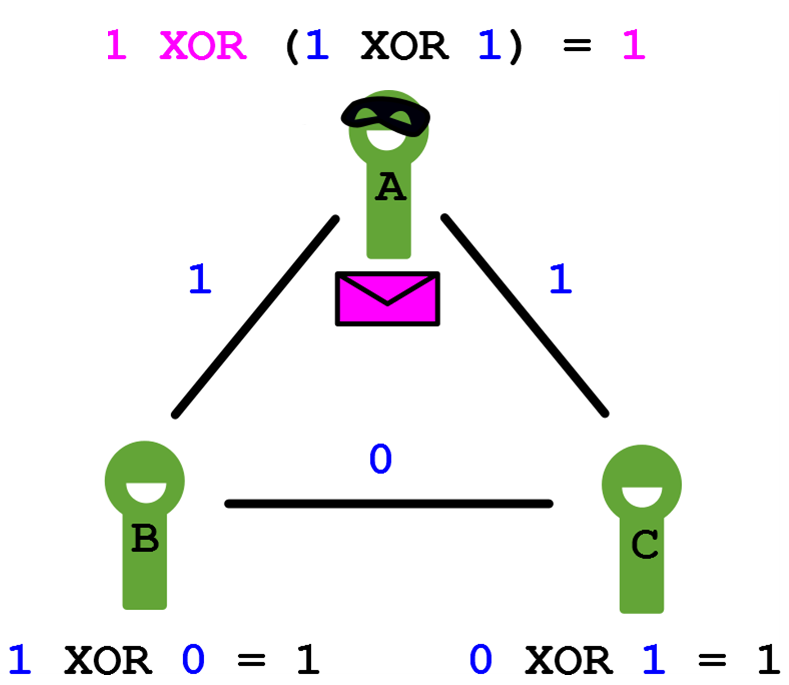
\includegraphics[scale=.30]{DCNet.png} \caption{Working of Dining Cryptographers Networks}
\label{fig:DCNet}

\end{figure*}

Our system applications are currently limited due to several assumptions made during the design process. We assume that all nodes participating as senders or receivers are known, which is typically not true in a mobile environment where nodes can constantly be joining or leaving the network. Furthermore, during pairwise communication, the choosing the leader based on ID value is not trivial when this information is private. Finally, we assume that there is no packet loss. In practical applications, packet loss is expected and will cause delay in the DC-net rounds of sharing messages.
 
Each round of the DC-net is composed of several sequential stages. The system must wait until all participants complete the current stage tasks before everyone can proceed onto the next stage. The three stages repeated for each bit in the message string are listed below:
\begin{itemize}
\item All nodes have pairwise communication with their neighboring nodes and the one with the higher ID generates a random bit privately shared between the two.
\item Each node pair establishes a secret shared key in a Diffie Hellman exchange.
\item All nodes XOR their known bits and publicly shares the result with the network. The sender XORs its announcement with the message bit.
\end{itemize}
All these announcements are XORed together and the result is received by all nodes. This result is the message. Since there is no association of the message with the sender, the sender remains anonymous. 


\subsection{Niji Protocol}
Every message that we send using our protocol is sent using the DCNet principle. The messages can be of three types: MSG (Initial message), SET (Share the AES key encrypted using the public key of the sender) and REP (reply message encrypted using AES key). Every node has a public private key pair. We initially choose a leader and this leader will send a message to every other node. This message contains the message type MSG, a message ID, the message and its public key. 

The node that wants to reply to this message first needs to establish an AES key with the sender node. So, this node sends a message containing the message type SET, the same message ID, an AES key. It encrypts this message using the public key of the sender so that only the sender can decrypt this message using its private key. Once this message is decrypted by the sender node, it stores the AES key from this message in its database. Now, for further communication between these two nodes, this AES key is used for encryption. However, we still keep the communication anonymous using DCNets. Once the AES key is established for communication, the messages that are sent will have the prefix REP attached to the message which indicates that these are normal messages exchanged between the sender and the receiver. 

When all the nodes receive the REP message, since none of the nodes know who it is from or who it is meant for, all of them try to decrypt the message using all the AES keys in their database. So, a brute force approach is used to decrypt the message. We propose a way of optimizing this and avoiding brute force later. 


\begin{figure*}
\centering
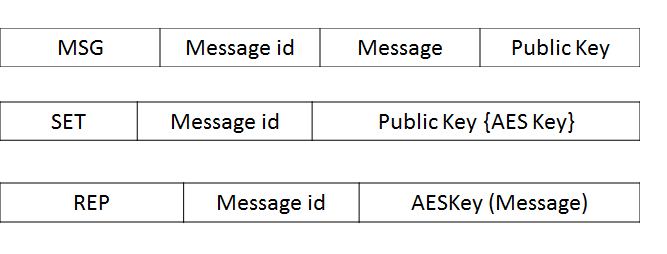
\includegraphics[scale=.45]{MSGFormat2.png} \caption{Message Format}
\medskip
\small
In a network of three nodes, each pair of nodes secretly share bits
\label{fig:DCNet}
\end{figure*}

\begin{figure*}
\centering
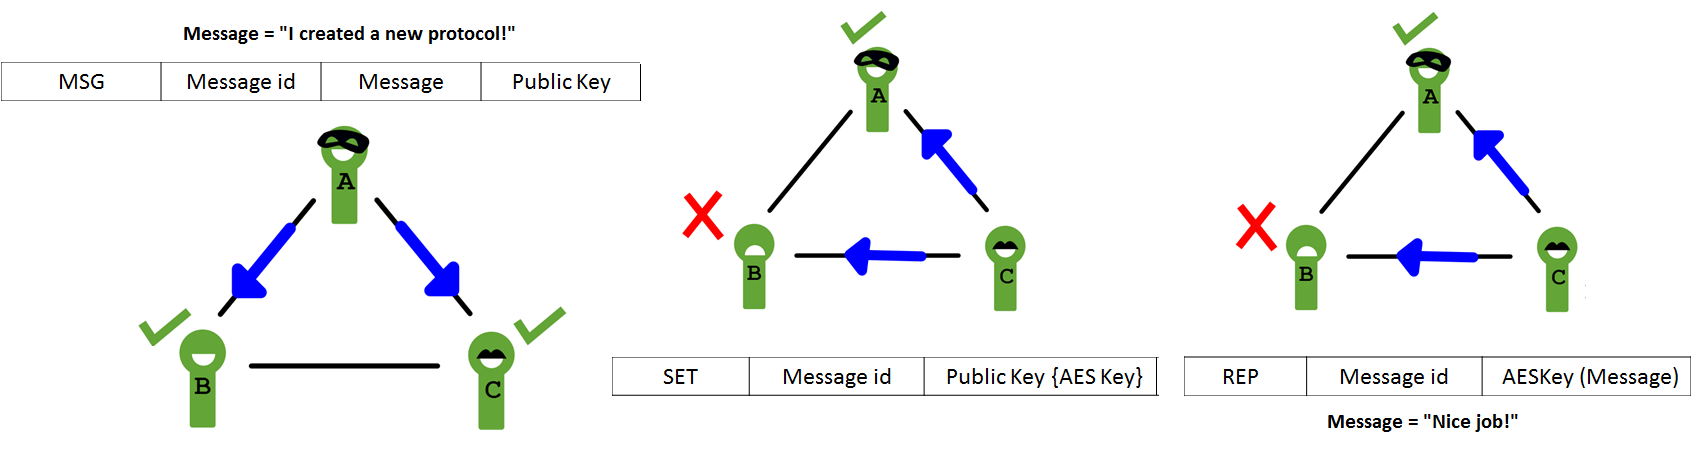
\includegraphics[scale=.40]{NIJI2.png} \caption{NIJI Working}
\medskip
\small
In a network of three nodes, each pair of nodes secretly share bits
\label{fig:NIJI}
\end{figure*}



\section{Implementation}
\vspace{1 mm}

We have simulated a network of variable number of nodes connected with WiFi. For transmission of packets we use UDP protocol for faster transmission. We have made the following assumptions while performing this experiment:
\begin{itemize}

\item Our network is assumed to have no packet loss or congestion. 
\item There are no malicious nodes
\item There is no churn in the network (i.e. no joining or leaving of nodes)
\item We choose the leader based upon node ID
\end{itemize}
We use the crypto++ library for encryption of messages. The crypto++ package needs to be integrated with ns-3 in order to be used. Once integrated, we can use the Diffie Hellman module for the random bit encryption and also the AES module for the encryption of the messages. It works smoothly and efficiently.  We have used the Simulator class ScheduleNow instruction to call the methods as and when required. For the keys, we use several data structures. Maps are used for storing corresponding information during Diffie Hellman key exchange. We also use a map to store the random bit and associate it with the other node with which it is shared. We use a random number generator to generate 0 or 1 with equal probability. The message to be sent can be hardcoded or passed by commandline. The message is converted into a stream of bits so that the transmission can be done using DCNets.  Before establishing the Diffie Hellman key, a public key and private key is generated at each node. While sending the DH (Diffie Hellman) public key we put the node ID in the tag portion of the packet so that the receiver nodes can associate the key with that particular node. 


\section{Experimental Results}
\vspace{1 mm}

To quantify the performance of the DC-net protocol, experiments were completed using the ns-3 network simulator. When the number of nodes is held constant, the total latency required to complete the messaging rounds grows linearly with the message length in bits, as shown in Fig. a. Furthermore, the number of packets sent and received each also demonstrates linear growth. Note that because there is no packet loss in the simulation, the number of packets sent equals the number of packets received. In a true mobile -network, the transmissions would not exhibit this ideal behavior, but instead experience packet drops.


Though the simulation shows linear growth in tests with a constant number of nodes, the total latency and packet count increases exponentially as the number of nodes grows. Fig shows the simulation results for two different constant message lengths. The data curve for tests when message length was 3 appear more flat due to the scaling when plotted along with the tests when message length was 50; however, when plotted individually, the tests when message length was 3 was also distinctively exponential. In a mobile platform, the number of nodes could easily grow beyond thousands of users. Thus, to make this protocol practical for real world use, optimization techniques need to be implemented to bring the runtime closer to linear growth.

\section{Conclusion}
\vspace{1 mm}

We have been able to achieve sender anonymity as well as receiver anonymity with our protocol. We have proved the anonymity using the DCNet principle. Also, we will be able to scale this to any number of nodes in the network. In our future work, we propose to consider mobile networks and take into account packet loss and congestion. Also, we plan to make several optimizations.  Instead of generating a new shared secret bit for every round, we intend to use a pseudo random generator which will generate a bit string of length equal to the message length. This will certainly reduce the time taken for each round and will improve the performance. We also plan to avoid brute force decryption of the receivers by using a prefix for every message. This will reduce the time taken by the receiver in decryption because it will not have to try decrypting the message with all its AES keys.

With the means of anonymous communication, there the is possibility that individuals or organizations could abuse this protocol for controversial applications. For example, criminals could plan attacks without being discovered by law enforcement. Political dissenter could exchange ideas and coordinate revolts against the government.

There are several existing mobile applications that claim to provide an anonymous messaging channel. For example, Secret, Confide, and most notably, Whisper. However, these applications store message data on the backend. The Niji protocol in unique in that it demonstrates provable, scalable anonymity in the mobile cloud.

\section{Future Work}
\vspace{1 mm}

In terms of future work, we intend to develop optimization techniques described previously to make NIJI practical for mobile cloud. In mobile cloud, users constantly enter or leave the network resulting in node churns. Thus, we want to understand the impact of packet loss, node churns and throughput.  

We plan to study the feasibility of various functions such as
\begin{itemize}
\item Advertise and form a private group of nodes to start anonymous communication.
\item Join existing DCnet groups.
\item Determine optimum group size.
\end{itemize}

In the future, we plan to integrate the NIJI protocol with Android and iOS platforms for public use. This application could be commercialized because the functionality provided is unique from existing applications that also address anonymity. For example, 

\section{Related Work}
\vspace{1 mm}


\section{Social Impact}
\vspace{1 mm}

\begin{thebibliography}{1}

\bibitem{torpir} P. Mittal, F. Olumofin, C. Troncoso, N. Borisov, and  I.  Goldberg {\em PIR-Tor: Scalable Anonymous Communication Using Private Information Retrieval} 20th USENIX Security Symposium, pages 475–490, 2011.

\bibitem{hubaux} M. Raya and J.-P. Hubaux. "The Security of Vehicular Ad Hoc Networks",  Wksp. Security in Ad hoc and Sensor Networks (SASN),  2005.

\bibitem{metrics} The Tor Project. Tor metrics portal, February 2011. http://metrics.torproject.org/..

\bibitem{stem} {\em https://stem.torproject.org/}

\bibitem{core} {\em http://www.nrl.navy.mil/itd/ncs/products/core}

\bibitem{torperf} {\em https://gitweb.torproject.org/torperf.git}

\bibitem{webmixes} O. Berthold, H. Federrath, and S. Kopsell. Web mixes: a system for anonymous and unobservable internet access. In International workshop on Designing privacy enhancing technologies:  design issues in anonymity and unobservability, 2001

\bibitem{anonymizer} J. Boyan. The anonymizer: Protecting user privacy on the web. Computer-Mediated Communication Maga- zine, 4(9), 1997.

\bibitem{or} R. Dingledine, N. Mathewson, and P. Syverson. Tor: The second-generation onion router.  In USENIX Se- curity, 2004.

\bibitem{anon} H. Federrath. Project: An.on - anonymity.online: Protection of privacy on the internet.  {\em http://anon.inf.tu-dresden.de/ }

\bibitem{goodin} D. Goodin.  Tor at heart of embassy passwords leak.
The Register, September 10 2007.

\bibitem{csf} A. Johnson and P. Syverson. More anonymous onion routing through trust. In IEEE CSF, 2009.

\bibitem{unobservability} P. Syverson, G. Tsudik, M. Reed, and C. Landwehr.
Towards an analysis of onion routing security. Workshop on Design Issues in Anonymity and Unobservability, 2000.

\bibitem{tor} {\em http://www.torproject.org/}

\end{thebibliography}


\end{document}
